\chapter{Implementacja}

W niniejszym rozdziale przedstawiono szczegóły implementacji systemu zarządzania wizytami lekarskimi, obejmujące strukturę projektu, zastosowane technologie oraz przykładowe fragmenty kodu źródłowego.

\section{Struktura projektu}

Projekt został zrealizowany zgodnie z podejściem warstwowym, obejmując następujące główne warstwy:

\begin{itemize}
\item \textbf{Warstwa danych} -- odpowiedzialna za komunikację z bazą danych PostgreSQL z wykorzystaniem JDBC,
\item \textbf{Warstwa logiki aplikacji} -- zarządzająca procesami biznesowymi, walidacją danych oraz obsługą wyjątków,
\item \textbf{Warstwa prezentacji} -- implementująca graficzny interfejs użytkownika (GUI) w technologii Swing.
\end{itemize}

\section{Technologie}

W projekcie wykorzystano następujące technologie:
\begin{itemize}
\item \textbf{Język Java 17} -- jako podstawowy język programowania,
\item \textbf{Swing} -- do stworzenia graficznego interfejsu użytkownika,
\item \textbf{PostgreSQL} -- jako system zarządzania bazą danych,
\item \textbf{JDBC} -- technologia do komunikacji z bazą danych,
\item \textbf{LaTeX} -- narzędzie do przygotowania dokumentacji.
\end{itemize}

\section{Kluczowe klasy}

Poniżej przedstawiono kluczowe klasy oraz ich role w systemie:

\begin{itemize}
\item \textbf{Doctor, Patient, Person} -- reprezentujące podstawowe jednostki w systemie,
\item \textbf{Visit} -- zarządzająca danymi dotyczącymi wizyt,
\item \textbf{User} -- obsługująca użytkowników systemu, ich logowanie oraz autoryzację,
\item \textbf{DoctorDAO, PatientDAO, VisitDAO} -- klasy zapewniające dostęp do danych z bazy.
\end{itemize}

\clearpage
\section{Przykładowe fragmenty kodu}

\subsection{Klasa Doctor}
\begin{lstlisting}[style=javaStyle,caption={Klasa reprezentująca lekarza — rozszerzenie klasy Person}]
public class Doctor extends Person {
        private String specialization;

        public Doctor(int id, String firstName, String lastName, String phone, String email, String specialization) {
            super(id, firstName, lastName, phone, email);
            this.specialization = specialization;
        }

        @Override
        public String getInfo() {
            return "Lekarz: " + firstName + " " + lastName + " - " + specialization;
        }

        public String getSpecialization() {
            return specialization;
        }

        public void setSpecialization(String specialization) {
            this.specialization = specialization;
        }

        @Override
        public String toString() {
            return firstName + " " + lastName + " - " + specialization;
        }

    }
\end{lstlisting}

\subsection{Metoda logowania użytkownika}
\begin{lstlisting}[style=javaStyle, caption={Metoda logowania użytkownika z wykorzystaniem JDBC}]
 public User login(String login, String password) {
        String sql = "SELECT * FROM users WHERE login = ? AND password = ?";

        try (Connection conn = DatabaseConnection.getConnection();
             PreparedStatement stmt = conn.prepareStatement(sql)) {

            stmt.setString(1, login);
            stmt.setString(2, password);

            try (ResultSet rs = stmt.executeQuery()) {
                if (rs.next()) {
                    return new User(
                            rs.getInt("id"),
                            rs.getString("login"),
                            rs.getString("password"),
                            rs.getString("role"),
                            rs.getObject("patient_id") != null ? rs.getInt("patient_id") : null
                    );
                }
            }

        } catch (SQLException e) {
            e.printStackTrace();
        }
        return null; //login lub hasło nie prawidłowe
    }
\end{lstlisting}

\section{Obsługa wyjątków i walidacja}
Aplikacja posiada zaimplementowaną obsługę wyjątków, mającą na celu zapewnienie stabilności oraz poprawności działania systemu. Poniżej przedstawiono przykładowe wyjątki wraz z fragmentami kodu oraz komunikatami wyświetlanymi użytkownikowi.

\subsection{Niepoprawne dane logowania}

W przypadku próby logowania przy użyciu błędnego loginu lub hasła wyświetlany jest odpowiedni komunikat błędu (Rys. \ref{fig:falseLogin}).

\begin{figure}[H]
\centering
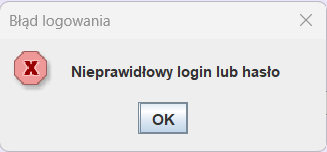
\includegraphics[width=0.5\textwidth]{figures/FalseDataforLogin.png}
\caption{Komunikat błędu - niepoprawne dane logowania}
\label{fig:falseLogin}
\end{figure}

Przykładowy fragment kodu:
\begin{lstlisting}[style=javaStyle, caption={Obsługa błędnego logowania — komunikat dla użytkownika}]
 if (user != null) {

    dispose();

        if (user.isSecretary()) {
            new SecretaryMainMenu().setVisible(true);
            } else if (user.isPatient()) {
                    PatientDAO patientDAO = new PatientDAO();
                    Patient patient = patientDAO.getPatientById(user.getPatientId());
                    if (patient != null) {
                    new PatientMainMenu(patient).setVisible(true);
                        } else {
                            JOptionPane.showMessageDialog(null, "Błąd: nie znaleziono danych pacjenta!", "Błąd", JOptionPane.ERROR_MESSAGE);
                        }
                    }
                }else {
                    JOptionPane.showMessageDialog(null, "Nieprawidłowy login lub hasło", "Błąd logowania", JOptionPane.ERROR_MESSAGE);
                }
\end{lstlisting}

\subsection{Istniejący login podczas rejestracji}

Przy próbie utworzenia nowego użytkownika z loginem, który już istnieje w bazie danych, aplikacja wyświetli stosowny komunikat (Rys. \ref{fig:loginExists}).

\begin{figure}[H]
\centering
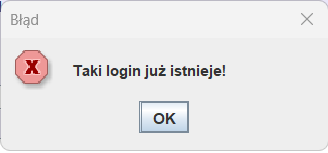
\includegraphics[width=0.4\textwidth]{figures/ThisLoginAlrExists.png}
\caption{Komunikat błędu - istniejący login}
\label{fig:loginExists}
\end{figure}

Przykładowy fragment kodu:
\begin{lstlisting}[style=javaStyle, caption={Walidacja unikalności loginu podczas rejestracji użytkownika}]
 public boolean loginExists(String login) {
        String sql = "SELECT 1 FROM users WHERE login = ?";
        try (Connection conn = DatabaseConnection.getConnection();
             PreparedStatement stmt = conn.prepareStatement(sql)) {
            stmt.setString(1, login);
            ResultSet rs = stmt.executeQuery();
            return rs.next();
        } catch (SQLException e) {
            e.printStackTrace();
        }
        return false;
    }    
/-----------------------------------------------------------------------\

 if (dao.loginExists(login)) {
            JOptionPane.showMessageDialog(null, "Taki login już istnieje!", "Błąd", JOptionPane.ERROR_MESSAGE);
            return;
        }

\end{lstlisting}

\subsection{Konflikt terminów wizyt}

Próba rezerwacji wizyty u lekarza w terminie, który koliduje z inną wizytą (z marginesem ±30 minut), powoduje wyświetlenie komunikatu o konflikcie (Rys. \ref{fig:visitConflict}).

\begin{figure}[H]
\centering
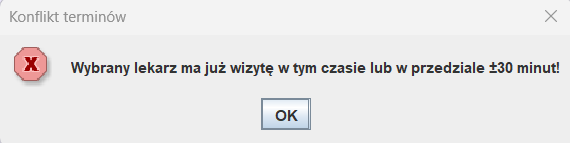
\includegraphics[width=0.6\textwidth]{figures/VisitKonflict.png}
\caption{Komunikat błędu - konflikt terminów wizyt}
\label{fig:visitConflict}
\end{figure}

Przykładowy fragment kodu:
\begin{lstlisting}[style=javaStyle, caption={Walidacja konfliktów wizyt ±30 minut u danego lekarza}]
public boolean hasDoctorConflict(int doctorId, LocalDateTime dateTime) {
    String sql = "SELECT COUNT(*) FROM visits WHERE doctor_id = ? AND ABS(EXTRACT(EPOCH FROM (visit_date - ?))) < 1800";

    try (Connection conn = DatabaseConnection.getConnection();
         PreparedStatement stmt = conn.prepareStatement(sql)) {

        stmt.setInt(1, doctorId);
        stmt.setTimestamp(2, Timestamp.valueOf(dateTime));

        ResultSet rs = stmt.executeQuery();
        if (rs.next()) {
            return rs.getInt(1) > 0;
        }
    } catch (SQLException e) {
        e.printStackTrace();
    }
    return false;
}

\end{lstlisting}

Powyższe przykłady stanowią tylko wybrane przypadki obsługi wyjątków w aplikacji. W projekcie zaimplementowano także inne wyjątki, takie jak błędy połączenia z bazą danych, walidacja danych wejściowych i inne komunikaty błędów użytkownika.


